
%


\section{Tools}\label{sec:tools}

\renewcommand{\kapitelautor}{Autor: Nils Hubmann}

\subsection{Jira}\label{subsec:jira}
%

\begin{coolQuote}
Jira ist eine Webanwendung, die sich im Laufe der Zeit zum Marktstandard in den Bereichen Projektmanagement, Aufgabenmanagement und Fehlerverwaltung entwickelt hat.
Insbesondere für die Softwareentwicklung ist Jira ein hervorragendes Tool, welches Arbeitsschritte und die Zusammenarbeit in kleinen oder größeren Teams deutlich erleichtern kann.
\end{coolQuote}
\zid{Jira}

Jira ist ein Softwaretool, das im Fall von \ff als Scrum Planungssoftware verwendet wurde.
Es besteht aus einem Product Backlog, in dem alle Tasks in Form von Epics und User Stories abgelegt sind.
Dieser wurde durch den Product Owner gepflegt, um Fortschritte zu überwachen und die Einträge zu priorisieren.
Für die einzelnen User Stories gab es Verantwortliche, die für die Fertigstellung zuständig waren.

%\begin{figure}[H]
%    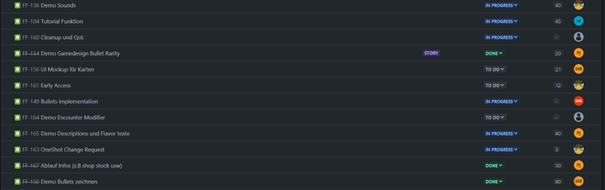
\includegraphics[width=\textwidth]{Backlog.png}
%    \caption{Backlog}
%\end{figure}

\subsection{Trello}\label{subsec:Trello}
%
Die Software Trello ist ein Projektmanagement Tool im Kanban Stil.
Es stellt ein Board dar, welches mit Karten befüllt wird.
Das Board ist in Spalten unterteilt, welche zur Kategorisierung oder zur Fortschrittseinteilung genutzt werden können.
Außerdem können Personen zu den Tasks zugewiesen werden, Aufwandseinschätzungen zugeordnet und Zeit getrackt werden.
Es ermöglicht eine einfache Übersicht durch die einfache simple Darstellung.

Das Team hat sich für Trello als internes Kanbanboard entschieden, da es damit aus vorherigen Projekten vertraut war und mit Jira nicht zurechtkam.
Einerseits ist Jira aus Sicht des Teams zu kompliziert und umfangreich.
Trello wurde nur als zur Übersicht über das Kanbanboard und zum Timetracking genutzt, während die standardmäßige Verwaltung der User Stories nach wie vor auf Jira stattfand.
Hierfür wurden die Tasks zusätzlich in Trello erstellt und darauf Zeit getracked.
Außerdem ist das Zeittracking in Jira mit Plugins wie Clockify äußerst umständlich und erschwert auch das mobile Zugreifen über das Telefon, was bei Trello druch eine App erleichtert wird.
Das Zeittracking ist innerhalb von Trello mit dem Tool Everhour passiert und konnte den Aufgaben zugeordnet werden.

\begin{figure}[H]
    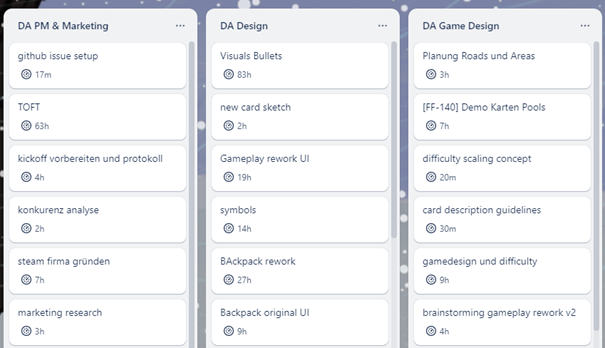
\includegraphics[width=\textwidth]{Trello_log.png}
    \caption{Trello}
\end{figure}

\subsection{Discord}\label{subsec:Discord}
Discord ist eine Kommunikationsplattform, die primär zur internen Kommunikation verwendet wurde, da sie viele Möglichkeiten der Kommunikation kombiniert.
Es sind sogenannte Voice Channels vorhanden, welche es den Teammitgliedern erlauben, zusammen zu arbeiten und sich während der Arbeit auszutauschen.
Es gibt Textkanäle, die das Versenden von Nachrichten, Informationen oder Dateien ermöglichen.
Außerdem dient es als soziale Plattform, um sich eine Community aufzubauen.\zit{Discord}

Intern ist die Wahl auf Discord gefallen, da alle Teammitglieder mit der Plattform vertraut sind.
Außerdem bietet sie dem Team den notwendigen Umfang, um die Zusammenarbeit zu vereinfach.
Sie verfügt über alle notwendigen Features, wie Sprachkanäle mit Bildschirmübertragungsfunktion, Textkanäle und ist auf internen Austausch ausgelegt.

\begin{figure}[H]
    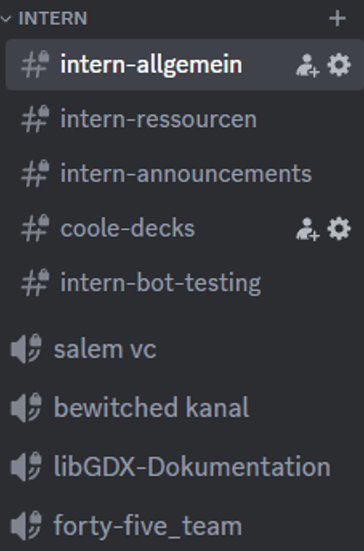
\includegraphics{Discord.png}\caption{Discord}
    \caption{Discord}
\end{figure}
%

% resets author
\renewcommand{\kapitelautor}{}
